\documentclass[a4paper,twoside]{scrbook}

%\usepackage{xcolor}
\usepackage{minted}
\newcommand{\q}[1]{\mintinline{latex}{#1}}

% https://ctan.mirrors.hoobly.com/macros/latex/contrib/titlesec/titlesec.pdf
% https://tex.stackexchange.com/questions/27411/small-caps-and-bold-face
\usepackage{bold-extra}
\usepackage{titlesec}
\titleformat{\section}
  {\bfseries\scshape}{Example \thesection}{1em}{}

\titleformat{\subsection}
  {\bfseries}{}{0em}{}

\usepackage{amsmath}
\usepackage{verbatim}


% https://tex.stackexchange.com/questions/229309/pdf-figure-will-not-scale
\usepackage{graphicx}


% https://www.nicholasnadeau.com/post/2018/08/admonition-blocks-making-your-documentation-stand-out/
% https://mirrors.rit.edu/CTAN/graphics/awesomebox/awesomebox.pdf
\usepackage{lipsum}
\usepackage{awesomebox}
\usepackage{alertmessage}

% https://tex.stackexchange.com/questions/504154/how-can-i-get-footnotes-in-awesomebox
\usepackage{footnote}
\makesavenoteenv{tabular}
\usepackage[bottom]{footmisc}
\usepackage{perpage} %the perpage package
\MakePerPage{footnote} %the perpage package command

% hyperlink
\usepackage{hyperref}
\hypersetup{
    colorlinks=true,
    linkcolor=blue,
    filecolor=magenta,      
    urlcolor=cyan,
    pdftitle={Overleaf Example},
    pdfpagemode=FullScreen,
    }
\urlstyle{same}

\newcounter{example}[section]
\newenvironment{example}[1][]{\refstepcounter{example}\par\medskip  
   \noindent \textbf{Example~\theexample. #1} \rmfamily \vspace{3mm}}{\medskip}



\setlength\parindent{0pt}

\begin{document}
\title{q for qbies}
\author{David Han}
\frontmatter
\maketitle
\setcounter{tocdepth}{1}
\tableofcontents
\mainmatter

\chapter{Mathematics}

\section{Identity Matrix}
\label{example:LinearInterpolcation}

In linear algebra, an identity matrix of size 3 looks like:

$$
\left[
\begin{matrix}
1 & 0 & 0\\
0 & 1 & 0\\
0 & 0 & 1\\
\end{matrix}
\right]
$$


\subsection{Implementation}
Below is the function to create an identity matrix of any given size $n$.

\begin{minted}[samepage,frame=single,framesep=10pt,xleftmargin=10pt,linenos]{q}
.qe.math.identity:{[n]
  `float$v=/:v:til n
  };
\end{minted}

And the output \q{.qe.math.identity[4]} is

\begin{verbatim}
1 0 0 0 
0 1 0 0 
0 0 1 0 
0 0 0 1 
\end{verbatim}


\subsection{Explanations}
Let's look at this function in details.

\begin{itemize}
\item \begin{minted}{q}
v:til n
\end{minted}
\q{til n} returns all integers from zero up to $n$, but not including $n$ and assigns the list of integers to variable \q{v}. Note that the assignment operator returns the result of the expression assigned to $v$, which is later used by other expression to the left.

\item \begin{minted}{q}
v=/:v
\end{minted}
The list \q{v} is compared with each element of itself. So the returned value is a list of list of boolean values. For example, when \q{v} is compared with $v_i$ where $i = 0, 1, \cdots, n-1$, a list of boolean values is returned and the $i^{th}$ element is \q{1b} and \q{0b} elsewhere. Let $m_{ij}$ denote the element $j$ of the inner list, which is the element $i$ of the outer list, then 

$$
m_{ij} = 
\begin{cases}
\enspace \q{1b} & \text{ if } i=j, \\
\enspace \q{0b} & \text{ else. }
\end{cases}
$$

\item The result is an $n$x$n$ matrix of boolean values, which is then casted to a matrix of floating point numbers. The boolean value \q{1b} is casted to \q{1f} and \q{0b} is casted to \q{0f}.
\end{itemize}


\subsection{Summary}

\begin{importantblock}
\textbf{Important Note}
\begin{itemize}
\item For some matrix operators like \q{mmu}, \q{inv} and \q{$}, the matrix entries must of \q{float} type, \emph{i.e.} \q{all 9h=type each m} must be true if \q{m} is a matrix.
\end{itemize}
\end{importantblock}

\begin{noteblock}
\textbf{Knowledge Points}
\begin{itemize}
\item Function \href{https://code.kx.com/q/ref/til/}{\q{til}} 
\item Return value of assignment operation\footnote{See section Syntax on this page: \url{https://code.kx.com/q/ref/assign/}}
\item Each right \href{https://code.kx.com/q/ref/maps/#each-left-and-each-right}{\q{/:}}
\item Type casting: \href{https://code.kx.com/q/ref/cast/}{\q{$}}
\item Matrix entries must be of \q{float} type
\end{itemize}
\end{noteblock}

\clearpage

\section{Linear Interpolation}
\label{example:LinearInterpolcation}

Linear interpolation is widely used to find the new value along the line determined by two data points. Figure \ref{fig:LinearInterpolation} shows how to find the linearly interpolated value from the two points $(x_0,y_0)$ and $(x_1,y_1)$ by the linear interpolant when $x_0 \le x \le x_1$

\begin{equation}
\label{eq:LinearInterpolation}
\begin{split}
L(x) &= y_0+\frac {y_1-y_0}{x_1-x_0} (x-x_0) \\
     &= \left(1-\frac{x-x_0}{x_1-x_0}\right)\cdot y_0 + \frac{x-x_0}{x_1-x_0}\cdot y_1 \\
	 &= (1-w) \cdot y_0 + w \cdot y_1
\end{split}
\end{equation}

where

$$
w = \frac{x-x_0}{x_1-x_0}
$$

Graphically,

\begin{figure}[h]
\centering
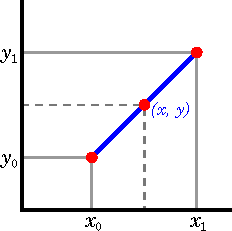
\includegraphics[width=8cm]{./figures/LinearInterpolation.pdf}
\caption{Linear interpolation}
\label{fig:LinearInterpolation}
\end{figure}


\subsection{Implementation}
In the implementation below, no linear extrapolation is performed for values outside the interval $[x_0, x_1]$. All the parameters of this function are simple numerical numbers. The first parameter is the $x$-coordinates of two data points and the second parameter is the $y$-coordinates of the two data points. The third parameter is the $x$-coordinate for the point to perform linear interpolation.

\begin{minted}[samepage,frame=single,framesep=10pt,xleftmargin=10pt,linenos]{q}
.qe.math.lerp:{[x;y;z]
  if[2<>count x;'"First argument must be a two-element list"];
  if[x[0]>x 1;'"First argument must be in ascending order"];
  if[not z within x;:$[z<x 0;y 0;y 1]];
  w:%[z-x 0;x[1]-x 0];
  (1-w;w) wavg y
  };
\end{minted}

\subsection{Explanations}

\begin{itemize}
\item Line 2 checks the number of elements in the first parameter. It must have two elements. Otherwise an error is thrown.
\item Line 3 checks whether the second element is not smaller than the first element in the first parameter. Otherwise, an error is thrown.
\item Line 3 returns the $y$-coordinate value if $x$-coordinate is not within the interval defined by the two points.
\item Line 5 computes the weight for the value to interpolate
\item Line 6 calculates the weighted average
\end{itemize}


\subsection{Summary}

\begin{importantblock}
\textbf{Important Note}
\begin{itemize}
\item The argument \q{x} must be in ascending order in this implementation.
\end{itemize}
\end{importantblock}

\begin{noteblock}
\textbf{Knowledge Points}
\begin{itemize}
\item Functions \href{https://code.kx.com/q/ref/if/}{\q{if}}, \href{https://code.kx.com/q/ref/count/}{\q{count}}, \href{https://code.kx.com/q/ref/within/}{\q{within}} and \href{https://code.kx.com/q/ref/wavg/}{\q{wavg}} 
\item The if-else like conditional selection: \href{https://code.kx.com/q/ref/cond/}{\q{$}}
\item Error signalling: \href{https://code.kx.com/q/ref/signal/}{\q{'}}
\end{itemize}
\end{noteblock}

\clearpage

\section{Piecewise Linear Interpolation}
\label{example:PiecewiseLinearInterpolcation}

The piecewise linear interpolation is an extension of the linear interpolation for two data points discussed in Example \ref{example:LinearInterpolcation}. It can be used to approximate any polynomial functions. Graphically,

\begin{figure}[h]
\centering
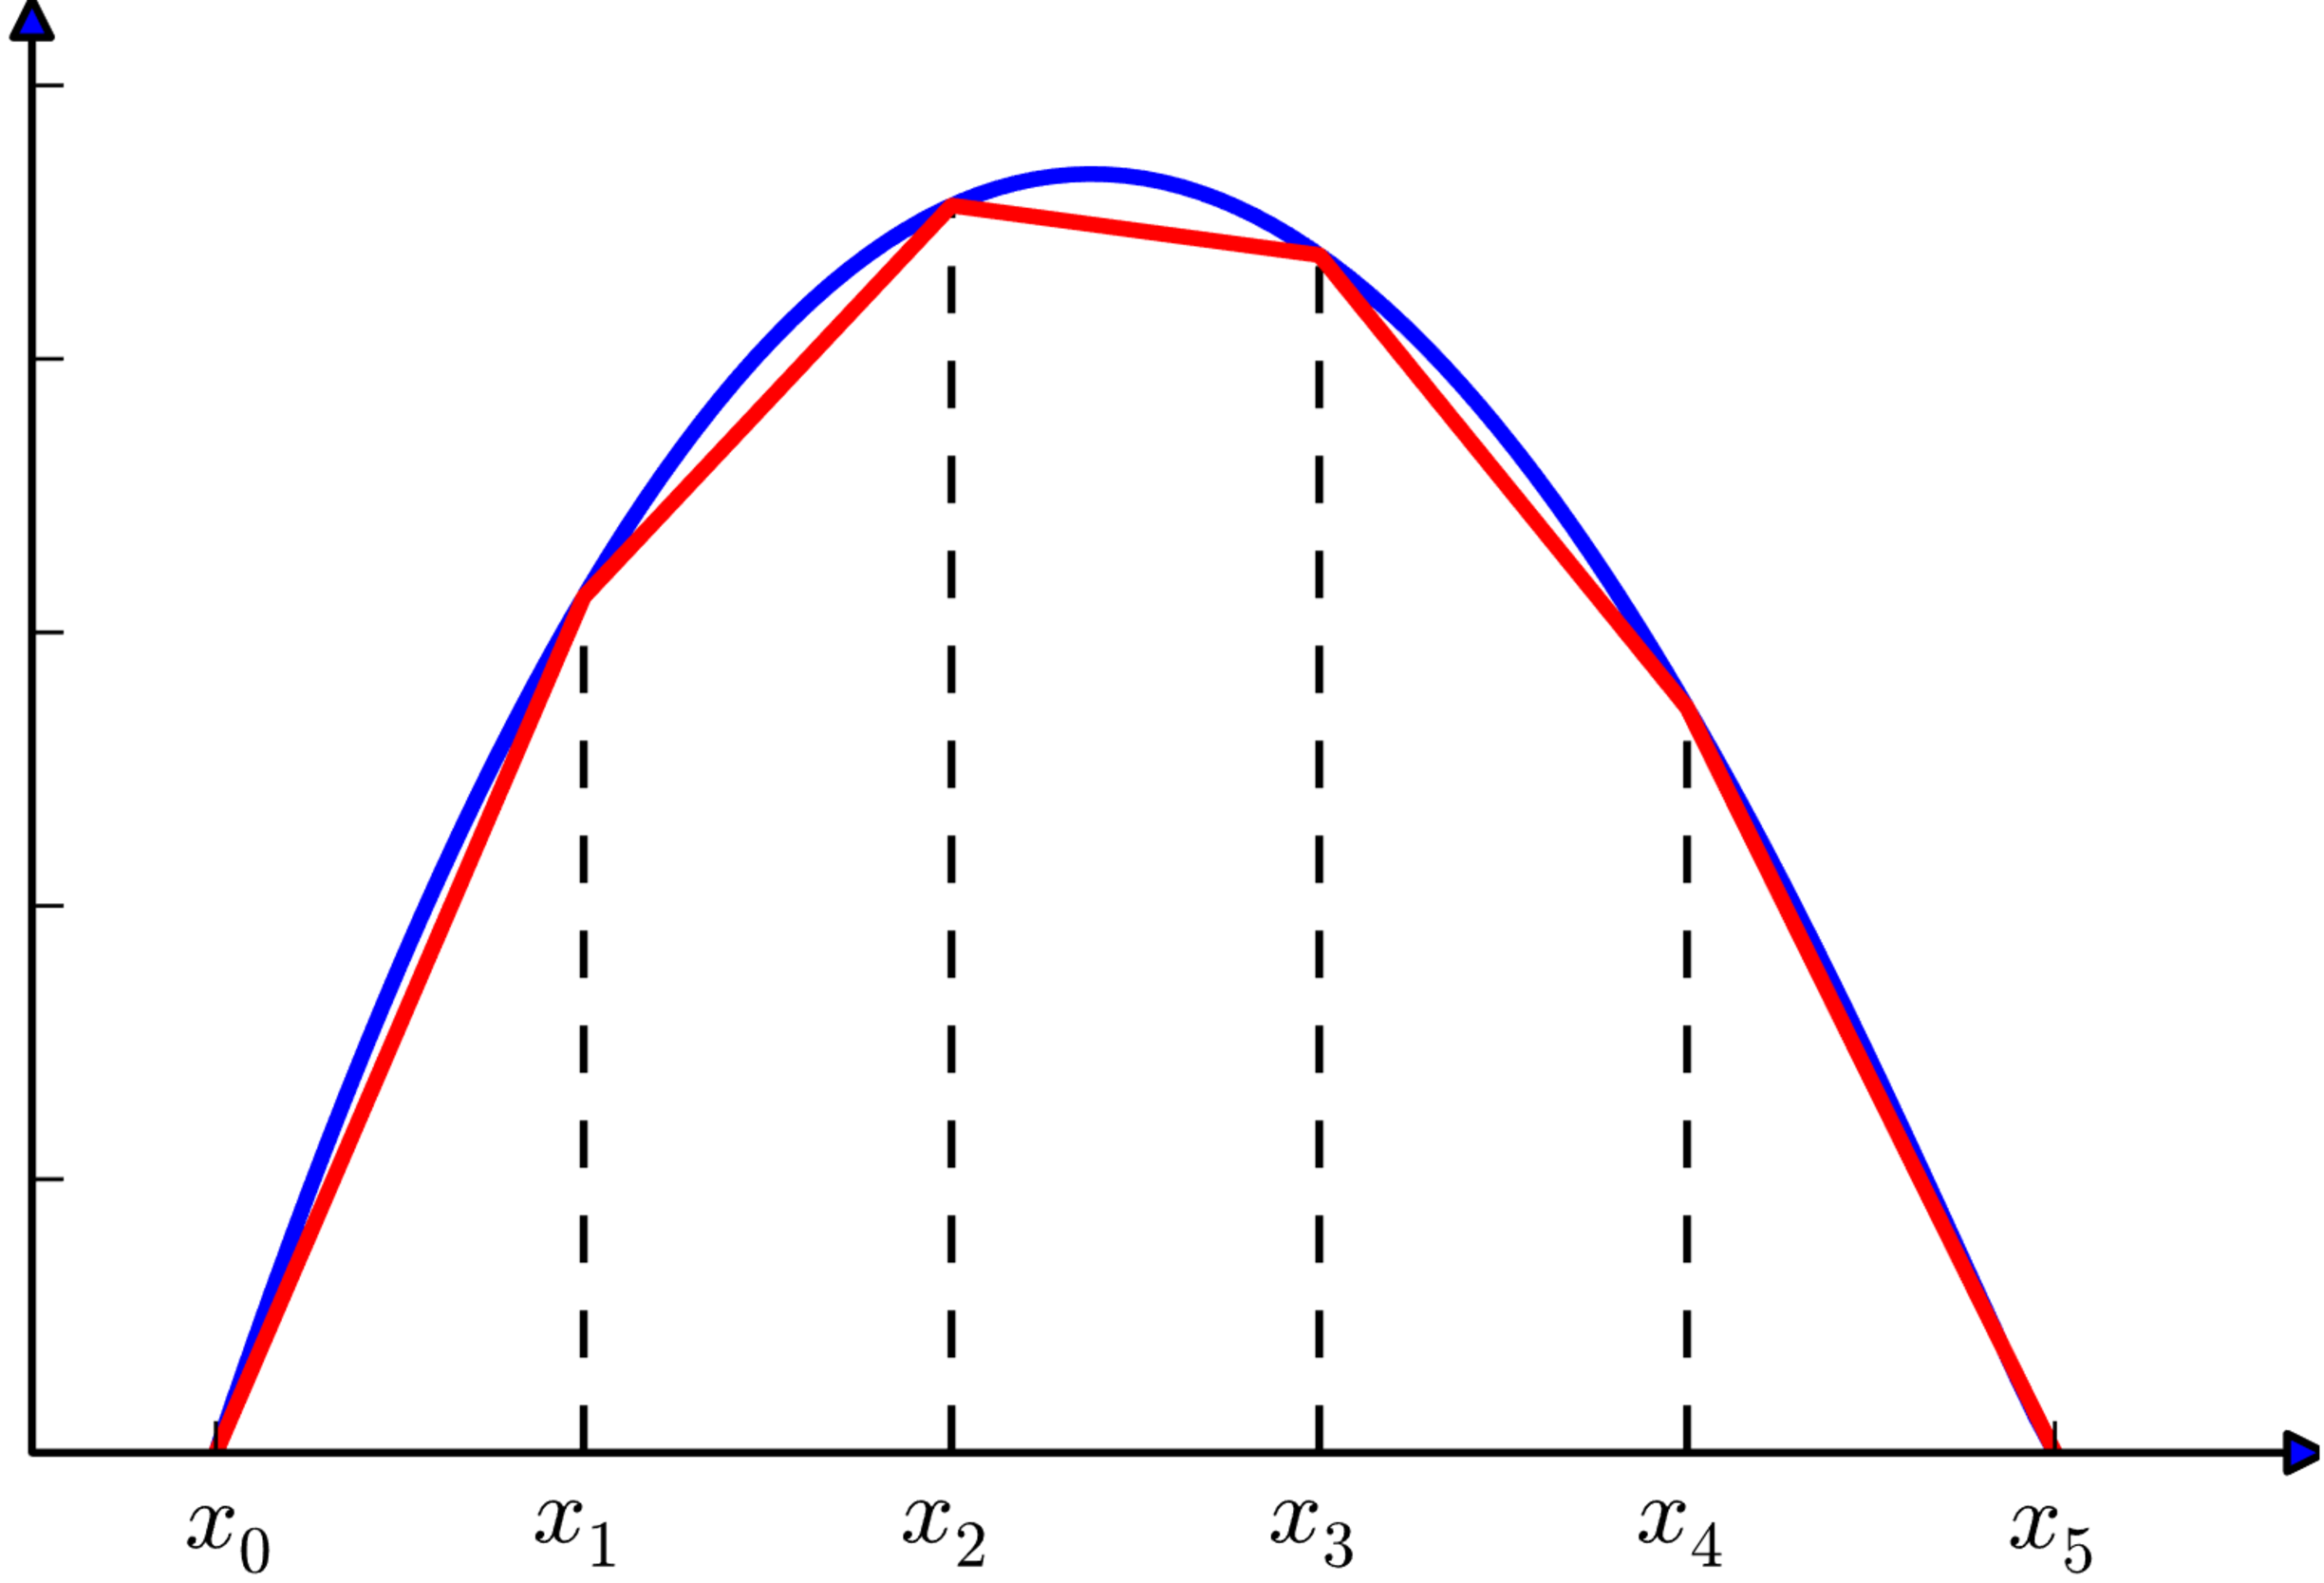
\includegraphics[width=10cm]{./figures/PiecewiseLinear.pdf}
\caption{Piecewise linear}
\label{fig:PiecewiseLinear}
\end{figure}

Suppose that we have $n$ data points: $(x_1, y_1), (x_2, y_2), \cdots, (x_i, y_i), \cdots (x_n, y_n)$ and the $x$-coordinate of the interpolation point is $z$. The piecewise linear interpolant is built upon the local linear interpolants.

$$
L(z) = 
\begin{cases}
\enspace L_1(z) & \text{ if } x_1 \le z < x_2, \\
\enspace L_2(z) & \text{ if } x_2 \le z < x_3, \\
\enspace \quad\vdots & \qquad\quad\vdots \\
\enspace L_i(z) & \text{ if } x_i \le z < x_{i+1}, \\
\enspace \quad\vdots & \qquad\quad\vdots \\
\enspace L_{n-1}(z) & \text{ if } x_{n-1} \le z < x_n,
\end{cases}
$$

where

$$
L_i(z) = \left(1-\frac{z-x_i}{x_{i+1}-x_i}\right) \cdot y_i + \frac{z-x_i}{x_{i+1}-x_i} \cdot y_{i+1}
$$

So once we find the interval $[x_i, x_{i+1})$ where the interpolation point falls into, we can simply call the function defined in Example \ref{example:LinearInterpolcation} to compute the interpolated value.

\subsection{Implementation}
The function belows takes three arguments with $n \ge 2$:

\begin{itemize}
\item \q{x} - a list of $x$-coordinates, \emph{i.e.} $x = (x_1, x_2, \cdots, x_i, \cdots, x_n)$
\item \q{y} - a list of $y$-coordinates, \emph{i.e.} $y = (y_1, y_2, \cdots, y_i, \cdots, y_n)$
\item \q{z} - the $x$-coordinate of the interpolation point
\end{itemize}

So there are $n$ data points in the above example and $(x_i,y_i)$ is the data point $i$.

\begin{minted}[samepage,frame=single,framesep=10pt,xleftmargin=10pt,linenos]{q}
.qe.math.pwlerp:{[x;y;z]
  if[all x=asc x;'"First argument must be in ascending order"];
  if[z>=last x;:last y];
  if[z<=first x;:first y];
  i:bin[`float$x;`float$z];
  x:@[x;(i;i+1)];
  y:@[y;(i;i+1)];
  .qe.math.lerp[x;y;z]
  };
\end{minted}


\subsection{Explanations}
In the implementation above,

\begin{itemize}
\item Line 2 checks whether the first argument is in ascending order. Otherwise, an error is thrown.
\item Line 3 checks whether the $x$-coordinate of the interpolation point is greater the largest $x$-coordinate of all data points. If so, return the $y$-coordinate of the last data point.
\item Line 4 checks whether the $x$-coordinate of the interpolation point is smaller the smallest $x$-coordinate of all data points. If so, return the $y$-coordinate of the first data point.
\item Line 5 finds the index of the interval where the interpolation point falls into. We also convert the two arguments of \q{bin} to \q{float} type to avoid potential \q{type} error.
\item Lines 6 and 7 narrow down the endpoints for the local interpolant.
\item Line 8 calls the linear interpolation function defined earlier.
\end{itemize}


\subsection{Summary}

\begin{importantblock}
\textbf{Important Note}
\begin{itemize}
\item The argument \q{x} must be in ascending order in this implementation.
\end{itemize}
\end{importantblock}

\begin{noteblock}
\textbf{Knowledge Points}
\begin{itemize}
\item Functions \href{https://code.kx.com/q/ref/if/}{\q{if}}, \href{https://code.kx.com/q/ref/all-any/#all}{\q{all}}, \href{https://code.kx.com/q/ref/asc/}{\q{asc}}, \href{https://code.kx.com/q/ref/first/#first}{\q{first}} and \href{https://code.kx.com/q/ref/first/#last}{\q{last}} 
\item Type casting: \href{https://code.kx.com/q/ref/cast/}{\q{$}}
\item Error signalling: \href{https://code.kx.com/q/ref/signal/}{\q{'}}
\item Binary search: \href{https://code.kx.com/q/ref/bin/}{\q{bin}}
\item Apply at index: \href{https://code.kx.com/q/ref/apply/#apply-at-index-at}{\q{@}}
\end{itemize}
\end{noteblock}


\clearpage

\section{Step Function}

A step function is a piecewise constant function as show in Figure \ref{fig:StepFunction}.

\begin{figure}[h]
\centering
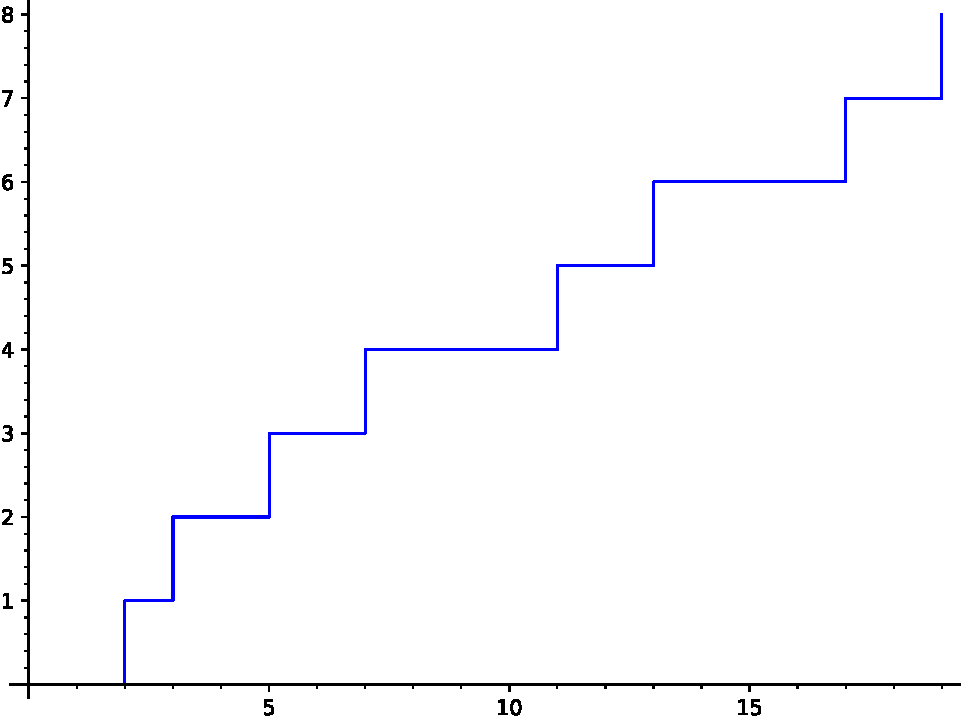
\includegraphics[width=8cm]{./figures/StepFunction.pdf}
\caption{Step function}
\label{fig:StepFunction}
\end{figure}

Mathematically,

$$
f(x) = 
\begin{cases}
\enspace c_0 & \text{ if } -\infty \le x < x_1, \\
\enspace c_1 & \text{ if } x_1 \le x < x_2, \\
\enspace \vdots & \qquad\quad\vdots \\
\enspace c_i & \text{ if } x_i \le x < x_{i+1}, \\
\enspace \vdots & \qquad\quad\vdots \\
\enspace c_n & \text{ if } x_n \le x < \infty,
\end{cases}
$$

A shopping mall is having its goods on sale. The discount rate varies and depends on the original marked price. The price discount table is as follows. For example, if an item has an original marked price of \$60, the sale price will have a $20\%$ off so you only need to pay \$48 for it.

\begin{center}
\begin{tabular}{l r } 
 \hline 
 Marked Price & Discount \\ [0.5ex] 
 \hline 
 $[0,10)$ & 5\% \\ [0.5ex] 

 $[10,30)$ & 10\% \\ [0.5ex] 

 $[30,50)$ & 15\% \\ [0.5ex]

 $[50,100)$ & 20\% \\ [0.5ex]

 $[100,200)$ & 30\% \\ [0.5ex]

 $[200,\infty)$ & 40\% \\
 \hline

\end{tabular}
\end{center}

\subsection{Implementation}
We write a function to compute the final price after discount for a given marked price. We propose two implementations.

\begin{minted}[samepage,frame=single,framesep=10pt,xleftmargin=10pt,linenos]{q}
// Implementation #1
.qe.math.finalPrice1:{[mp]
  prices:0 10 30 50 100 200;
  discounts:0.05 0.1 0.15 0.2 0.3 0.4;
  d:`s#prices!discounts;
  mp*1-d mp
  };
\end{minted}

Alternatively,
\begin{minted}[samepage,frame=single,framesep=10pt,xleftmargin=10pt,linenos]{q}
// Implementation #2
.qe.math.finalPrice2:{[mp]
  prices:0 10 30 50 100 200;
  discounts:0.05 0.1 0.15 0.2 0.3 0.4;
  mp*1-discounts prices bin mp
  };
\end{minted}

\subsection{Explanations}
In implementation \#1,

\begin{itemize}
\item Lines 3 and 4 define the price and discount lists
\item Line 5 creates a dictionary mapping from price thresholds to discount rate. Then a sorted attribute is applied to the keys of the dictionary. Setting a sorted attribute to a dictionary makes it a step function.
\item Line 6 first retrieve the discount rate for the given marked price and calculate the final price after discount.
\end{itemize}

In implementation \#2:

\begin{itemize}
\item Line 6 first finds the index of the price bucket where the marked price falls into and then retrieves the discount rate for the given marked price. It then calculates the final price after discount.
\end{itemize}

\subsection{Summary}

\begin{importantblock}
\textbf{Important Note}
\begin{itemize}
\item For a regular dictionary 
\begin{minted}{q}
d:10 20 30!0.1 0.2 0.3;
\end{minted}
\q{d[10]} gives $0.1$ but \q{d[11]} gives \q{0nf} since 11 is not a key of \q{d}.

\item For a dictionary with sorted attribute,
\begin{minted}{q}
d:`s#10 20 30!0.1 0.2 0.3;
\end{minted}
\q{d[10]} gives $0.1$ and \q{d[11]} also gives $0.1$ even though 11 is not a key of \q{d}. Because of the sorted attribute, \q{d} now is a step function and \q{d[x]} returns the value for the closest key which is smaller than \q{x}.
\end{itemize}
\end{importantblock}

\begin{noteblock}
\textbf{Knowledge Points}
\begin{itemize}
\item Set attribute: \href{https://code.kx.com/q/ref/set-attribute/}{x\#y}
\item Make a dictionary: \href{https://code.kx.com/q/ref/dict/#dict}{\q{x!y}}
\item Binary search: \href{https://code.kx.com/q/ref/bin/}{\q{bin}}
\end{itemize}
\end{noteblock}


\clearpage


\chapter{Dictionaries}

\section{Create a Dictionary}

There are multiple different ways to create a dictionary in q and I will explain each of them in this example. The first and foremost, the basic definition of a dictionary using \q{!}, \emph{i.e.} \q{x!y} or \q{![x;y]}.


\subsection{Basic method}
\begin{minted}[frame=single,framesep=10pt,xleftmargin=10pt,linenos]{q}
`a`b`c`d`e!5 4 3 2 1
\end{minted}

Or alternatively,
\begin{minted}[frame=single,framesep=10pt,xleftmargin=10pt,linenos]{q}
![`a`b`c`d`e;5 4 3 2 1]
\end{minted}


\subsection{Dot apply}
Here \q{.} applies an operator or function to a list of arguments. Line 1 uses function projection.

\begin{minted}[frame=single,framesep=10pt,xleftmargin=10pt,linenos]{q}
.[!](`a`b`c`d`e;5 4 3 2 1)
.[!;(`a`b`c`d`e;5 4 3 2 1)]
\end{minted}


\subsection{Over accumulator}
The \q{over} derives an accumulator from a binary function. In the example below, it basically performs two evaluations sequentially:
\begin{itemize}
\item the list \q{`a`b`c`d`e} is returned since it is the first element
\item In the second evaluation, the result of first evaluation becomes the left argument and the right argument is the second element from the list, \emph{i.e.} \q{5 4 3 2 1}
\end{itemize}
\begin{minted}[frame=single,framesep=10pt,xleftmargin=10pt,linenos]{q}
(!/)(`a`b`c`d`e;5 4 3 2 1)
\end{minted}


\subsection{Dot apply again}
This is basically the same as above except a few notable points:
\begin{itemize}
\item function \q{flip} is used to create a list of lists. In this case, the list has two elements and the first element will be used as key and the second element will be used value in the dictionary contruction. This is quite useful when you have a long list of keys/values and it is less error prone when a pair is used.
\item Line 1 is basically a prefix notation \q{v[x;y]} and line 2 uses an infix notation \q{x v y} where the operator \q{v} is \q{.} apply.
\end{itemize}
\begin{minted}[frame=single,framesep=10pt,xleftmargin=10pt,linenos]{q}
.[!] flip ((`a;5);(`b;4);(`c;3);(`d;2);(`e;1))
(!). flip ((`a;5);(`b;4);(`c;3);(`d;2);(`e;1))
\end{minted}


\subsection{Summary}

\begin{noteblock}
\textbf{Knowledge Points}
\begin{itemize}
\item Make a dictionary: \href{https://code.kx.com/q/ref/dict/#dict}{\q{x!y}}
\item Dot apply: \href{https://code.kx.com/q/ref/apply/}{\q{.}}
\item Over accumulator: \href{https://code.kx.com/q/ref/accumulators/#binary-values}{\q{/}}
\item Flip: \href{https://code.kx.com/q/ref/flip/}{\q{flip}}
\end{itemize}
\end{noteblock}

\clearpage

\section{Add a New Key to a Dictionary}

Suppose you have an existing dictionary \q{d} as follows:

\begin{minted}[frame=lines,framesep=10pt,xleftmargin=10pt]{q}
q) d:`firstName`lastName!`John`Chang
q) d
firstName| John
lastName | Chang
\end{minted}

Now we want to add another key to this dictionary to indicate the age, say, 
\begin{minted}[frame=lines,framesep=10pt,xleftmargin=10pt]{q}
q) d[`age]:30;
'type
    [0]  d[`age]:30;
                ^
\end{minted}
Unfortunately, \q{q} complains with a \q{type} error. This is because
\begin{itemize}
\item The existing dictionary is uniform, and
\item The value type of new item is different from the value type of the existing dictionary
\end{itemize}


\subsection{Mixed value types}
When the existing dictionary has mixed values, it is Okay to directly insert a new item.

\begin{minted}[frame=lines,framesep=10pt,xleftmargin=10pt]{q}
q) d2:`firstName`lastName`zip!(`John;`Chang;10583);
q) d2
firstName| `John
lastName | `Chang
zip      | 10583

q) d2[`age]:30; /add a new item
q) d2
firstName| `John
lastName | `Chang
zip      | 10583
age      | 30
\end{minted}


\subsection{Uniform value type}
When the value type of the new item is different from the value type of the existing dictionary, we can create a second dictonary with the new key and then merge this dictionary with the existing dictionary. For example

\begin{minted}[frame=lines,framesep=10pt,xleftmargin=10pt]{q}
q) d:`firstName`lastName!`John`Chang
q) d
firstName| John
lastName | Chang

q) d,enlist[`age]!enlist 30
firstName| `John
lastName | `Chang
age      | 30
\end{minted}


\subsection{Summary}
When the value type of a dictionary is not known in advance, the second approach provides a more robust way to insert a new entry to an existing dictionary.

\begin{noteblock}
\textbf{Knowledge Points}
\begin{itemize}
\item Make a list: \href{https://code.kx.com/q/ref/enlist/}{\q{enlist}}
\item Join: \href{https://code.kx.com/q/ref/join/}{\q{,}}
\end{itemize}
\end{noteblock}

\clearpage


\chapter{Execution Control}

\section{Conditional Selection}


\begin{minted}[samepage,frame=single,framesep=10pt,xleftmargin=10pt,linenos]{q}
// A form of the conditional:
("j"$a=b) foo/bar  / ?[a=b;foo bar;bar]
a:2;
b:1;
foo:{x*x};
bar:1 2 3;
("j"$a=b) foo/bar

select time,side,sign:(-1;1)[side=`buy] from trade

select time,side,sign:?[side=`buy;1;-1] from trade

$[a=b;`equal;`notequal]

\end{minted}


\clearpage


\chapter{File System}

\section{Check whether a path is a directory}

\begin{minted}[samepage,frame=single,framesep=10pt,xleftmargin=10pt,linenos]{q}
.qq.fs.isdir:{[path]
  not any (();path)~\:key path
  };
\end{minted}

\subsection{Summary}

\begin{noteblock}
\textbf{Knowledge Points}
\begin{itemize}
\item Objects in a folder: \href{https://code.kx.com/q/ref/key/#files-in-a-folder}{\q{key}}
\end{itemize}
\end{noteblock}

\clearpage

\section{Find Files Recursively}

\begin{minted}[samepage,frame=single,framesep=10pt,xleftmargin=10pt,linenos]{q}
.qlib.fs.isdir:{
  not any (();x)~\:key x
  };

.qlib.fs.walkdir:{[folder]
  folderContents:` sv/:folder,/:key folder;
  folders:folderContents where .qlib.fs.isdir each folderContents;
  files:folderContents except folders;
  files,.z.s each folders
  };
\end{minted}

\clearpage



\end{document}